\documentclass[11pt,a4paper]{article}
\usepackage[utf8]{inputenc}\usepackage[T1]{fontenc}\usepackage{mathptmx}\usepackage[scaled=0.9]{helvet}\usepackage{courier}
\usepackage[margin=2.3cm]{geometry}\usepackage{amsmath,amssymb}\usepackage{graphicx}
\usepackage{booktabs}\usepackage{listings}\usepackage{xcolor}\usepackage{fancyhdr}
\usepackage[hidelinks]{hyperref}\usepackage{caption}\usepackage{tikz}\usepackage{tabularx}\usepackage[section]{placeins}
\usetikzlibrary{positioning,arrows.meta}
\renewcommand{\contentsname}{Table des matières}
\renewcommand{\figurename}{Figure}\renewcommand{\tablename}{Tableau}
\pagestyle{fancy}\fancyhf{}
\lhead{\small Blombou -- Bouaboud -- Nanda -- Sissoko -- Ziani}\rhead{\small SIT213 -- Rapport Étape 4}\cfoot{\thepage}
\lstset{language=Java,basicstyle=\ttfamily\small,columns=fullflexible,breaklines=true,frame=single,backgroundcolor=\color{gray!6},
  keywordstyle=\color{blue!60!black}\bfseries,commentstyle=\color{green!40!black}\itshape,
  literate={é}{{\'e}}1{è}{{\`e}}1{à}{{\`a}}1{É}{{\'E}}1{ê}{{\^e}}1{ù}{{\`u}}1{ç}{{\c{c}}}1}
\newcommand{\EbNo}{E_b/N_0}
\newcommand{\cls}[1]{\texttt{#1}}
\sloppy\setlength{\parskip}{4pt}\setlength{\parindent}{0pt}
\begin{document}
\begin{titlepage}\centering
{\large IMT Atlantique -- FIP2A\\ Module SIT213\par}\vspace{3cm}
{\LARGE\bfseries Simulation d'une chaîne de transmission numérique\par}\vspace{0.6cm}
{\Large Rapport -- Étape 4\\[4pt]\normalsize Canal à trajets multiples et récepteur à filtre adapté\par}\vspace{2.5cm}
\begin{tabular}{rl}
Groupe : & B4 -- FIP2A\\[4pt]
Auteurs : & BLOMBOU Ethan\\ & BOUABOUD Anis-Melwan\\ & NANDA Laurent\\ & SISSOKO Mohamed Djoncounda\\ & ZIANI Mohamed Amine\\[4pt]
Date : & Septembre 2026
\end{tabular}\vfill
\end{titlepage}
\tableofcontents\newpage

%======================================================================
\section{Objectifs de l'étape 4}
L'énoncé de l'atelier découpe l'étape 4 en deux parties :
\begin{itemize}
  \item \textbf{4a} -- transmission non idéale avec un bruit « réel » : nous avons retenu les \textbf{trajets multiples}, décrits par la fiche de la séance 4. Le signal reçu est la somme du trajet direct et de copies retardées et atténuées :
  \[ r(n) = s(n) + \sum_{k=1}^{K} ar_k\, s(n - dt_k), \qquad K \le 5 ; \]
  \item \textbf{4b} -- les mêmes trajets multiples \textbf{plus} le bruit blanc gaussien de l'étape 3 : $r(n) = s(n) + \sum_k ar_k\,s(n-dt_k) + b(n)$.
\end{itemize}
Le rapport de l'étape 3 concluait par ailleurs que notre récepteur, qui décidait sur un seul échantillon par bit, perdait $10\log_{10}N \approx 14{,}8$~dB par rapport à l'optimum, et que l'intégration d'un récepteur optimal était la priorité avant le codage de canal. Cette étape réalise donc aussi le \textbf{récepteur à filtre adapté}. Les objectifs sont :
\begin{itemize}
  \item modéliser le canal à trajets multiples, avec ou sans bruit, et l'intégrer au simulateur via l'option \texttt{-ti} de la commande unique ;
  \item remplacer la décision sur l'échantillon central par un filtre adapté valable pour les trois formes d'onde ;
  \item mesurer le TEB dans chaque configuration et le confronter à une théorie exacte de la chaîne.
\end{itemize}

%======================================================================
\section{Chaîne implémentée}
\begin{figure}[htbp]\centering
\resizebox{\linewidth}{!}{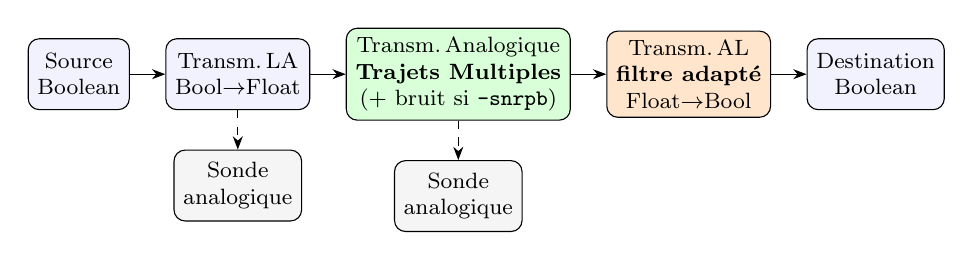
\begin{tikzpicture}[node distance=0.45cm,b/.style={draw,rounded corners,align=center,font=\footnotesize,minimum height=0.9cm,fill=blue!5},>=Stealth]
\node[b] (s) {Source\\Boolean};
\node[b,right=of s] (e) {Transm.\,LA\\Bool$\to$Float};
\node[b,right=of e,fill=green!15] (c) {Transm.\,Analogique\\\textbf{Trajets Multiples}\\(+ bruit si \texttt{-snrpb})};
\node[b,right=of c,fill=orange!20] (r) {Transm.\,AL\\\textbf{filtre adapté}\\Float$\to$Bool};
\node[b,right=of r] (d) {Destination\\Boolean};
\draw[->] (s)--(e); \draw[->] (e)--(c); \draw[->] (c)--(r); \draw[->] (r)--(d);
\node[b,below=0.5cm of e,fill=gray!8] (s1) {Sonde\\analogique}; \draw[->,dashed] (e)--(s1);
\node[b,below=0.5cm of c,fill=gray!8] (s2) {Sonde\\analogique}; \draw[->,dashed] (c)--(s2);
\end{tikzpicture}}
\caption{Chaîne de l'étape 4. En vert, le nouveau canal ; en orange, le récepteur modifié.}
\end{figure}
Le simulateur choisit le canal selon les options présentes :
\begin{center}\begin{tabular}{lll}\toprule
Options & Canal instancié & Perturbation\\\midrule
aucune & \cls{TransmetteurAnalogiqueParfait} & aucune\\
\texttt{-snrpb s} & \cls{TransmetteurAnalogiqueBruite} & bruit gaussien (étape 3)\\
\texttt{-ti dt ar ...} & \cls{TransmetteurAnalogiqueTrajetsMultiples} & échos seuls (4a)\\
\texttt{-ti dt ar ... -snrpb s} & \cls{TransmetteurAnalogiqueTrajetsMultiples} & échos puis bruit (4b)\\\bottomrule
\end{tabular}\end{center}
Le récepteur à filtre adapté est utilisé dans tous les cas analogiques.

%======================================================================
\section{Récapitulatif des modifications depuis l'étape 3}
\begin{center}\small\begin{tabularx}{\linewidth}{>{\raggedright\arraybackslash}p{4.6cm}X}\toprule
Élément & Modification\\\midrule
\texttt{TransmetteurAnalogique}\newline\texttt{TrajetsMultiples} & \textbf{Nouvelle classe.} Canal à trajets multiples, bruité ou non. Hérite de \cls{TransmetteurAnalogiqueBruite} (section~\ref{sec:heritage}).\\
\texttt{TransmetteurAnalogique}\newline\texttt{Bruite} & Le calcul du signal auquel on ajoute le bruit est isolé dans une méthode protégée \texttt{signalAvantBruit()}, que la sous-classe redéfinit. Comportement inchangé pour le canal gaussien seul.\\
\texttt{TransmetteurAnalogique}\newline\texttt{Logique} & \textbf{Récepteur à filtre adapté} : corrélation de tout le temps bit avec $g = s_1 - s_0$ au lieu d'un seuil sur l'échantillon central (section~\ref{sec:filtre}). Le constructeur reçoit désormais la forme d'onde.\\
\texttt{TransmetteurLogique}\newline\texttt{Analogique} & La génération d'un bit est extraite dans \texttt{formeBit(...)}, partagée avec le récepteur. Signal émis inchangé.\\
\texttt{Simulateur} & Nouvelle option \texttt{-ti} ; sélection du canal ; Eb/N0 infini sans \texttt{-snrpb} ; forme d'onde transmise au récepteur.\\
\texttt{runTests} & Section « Étape 4 » : 3 exécutions nominales et 3 tests d'erreur sur \texttt{-ti} ; renumérotation des commentaires (28 tests).\\
Tests JUnit & 22 tests ajoutés, 1 supprimé (option \texttt{-ebn0} hors spécification) : 96 tests, tous réussis.\\
\texttt{genDeliverable}, \texttt{README} & Archive \texttt{etape4} ; documentation de \texttt{-ti} et du filtre adapté, exemples remesurés.\\
\texttt{rapport/etape4/} & Script \texttt{courbesTEB.py} (simulations et théorie exacte) et outil \texttt{ExportSignal.java} qui produisent toutes les figures de ce rapport.\\\bottomrule
\end{tabularx}\end{center}

%======================================================================
\section{Prévisions avant simulation}
\subsection{Paramètres pertinents}
\begin{center}\begin{tabular}{lll}\toprule
Paramètre & Option & Rôle\\\midrule
Retard $dt_k$ d'un trajet indirect (échantillons) & \texttt{-ti} & position de l'écho par rapport au bit\\
Amplitude relative $ar_k$ & \texttt{-ti} & force de l'écho\\
Nombre de trajets (1 à 5) & \texttt{-ti} & nombre de couples $dt\ ar$\\
Rapport $\EbNo$ (dB) & \texttt{-snrpb} & bruit ajouté après les échos (4b)\\
Forme d'onde, $N$, amplitudes & \texttt{-form}, \texttt{-nbEch}, \texttt{-ampl} & forme du filtre adapté et du seuil\\\bottomrule
\end{tabular}\end{center}

\subsection{Résultats attendus}
\begin{itemize}
  \item \textbf{Filtre adapté.} Le TEB doit rejoindre la borne optimale : $Q\big(\sqrt{2\EbNo}\big)$ en NRZ antipodal et $Q\big(\sqrt{\EbNo}\big)$ en unipolaire, soit un gain de $10\log_{10}N \approx 14{,}8$~dB sur l'étape 3.
  \item \textbf{Trajets multiples sans bruit (4a).} L'écho d'un bit « déborde » sur les bits suivants : c'est de l'interférence entre symboles (IES). Tant qu'elle ne fait pas franchir le seuil, le TEB reste nul ; au-delà, le TEB passe brusquement à une fraction fixe (les suites de bits défavorables). Un écho retardé d'un bit entier ($dt = N$) doit être le plus gênant.
  \item \textbf{Trajets multiples et bruit (4b).} Pour un même $\EbNo$, le TEB doit être plus élevé qu'en l'absence d'écho, et d'autant plus que $ar$ est grand.
\end{itemize}

%======================================================================
\section{Modélisation du canal à trajets multiples}
\subsection{Modèle discret}
Chaque trajet indirect $k$ est une copie du signal émis, décalée de $dt_k$ échantillons et multipliée par $ar_k$ :
\[ r(n) = s(n) + \sum_{k=1}^{K} ar_k\, s(n - dt_k) \quad (+\,b(n)\ \text{en 4b}), \qquad s(m) = 0 \text{ pour } m < 0. \]
Avant le début d'un écho ($n < dt_k$), rien n'est encore réfléchi. La longueur du signal est conservée : la queue de l'écho du dernier bit est tronquée, ce qui est sans effet sur la décision.

\subsection{Option \texttt{-ti} de la commande unique}
La commande unique impose la syntaxe \texttt{-ti dt ar [dt ar ...]} : le retard (entier) vient avant l'amplitude (flottant), jusqu'à 5 couples, sans indiquer leur nombre. L'analyse lit des couples tant que l'argument suivant est un entier :
\begin{lstlisting}
} else if (args[i].matches("-ti")) {
    // Syntaxe : -ti dt1 ar1 [dt2 ar2 ...] (5 couples au maximum)
    simulationAnalogique = true;
    canalTrajetsMultiples = true;
    while (i + 1 < args.length && args[i + 1].matches("-?[0-9]+")) {
        i++;  int dt = Integer.parseInt(args[i]);      // dt >= 0, sinon erreur
        i++;  amplitudes.add(Float.parseFloat(args[i])); // ar manquant ou non flottant : erreur
        retards.add(dt);
    }
    if (retards.isEmpty() || retards.size() > NB_TRAJETS_MAX) throw new ArgumentsException(...);
\end{lstlisting}
Les arguments invalides lèvent une \cls{ArgumentsException} : \texttt{-ti} sans couple, plus de 5 couples, \texttt{ar} manquant ou non numérique, \texttt{dt} négatif ou hors des entiers. Un \texttt{dt} négatif est refusé car il désignerait un écho arrivant \emph{avant} le trajet direct ; il provoquait de plus un accès hors du tableau. Comme \texttt{-form} ou \texttt{-snrpb}, \texttt{-ti} active la simulation analogique.

\subsection{Implémentation par héritage}\label{sec:heritage}
Un canal à trajets multiples bruité est un canal gaussien dans lequel on insère une étape avant l'ajout du bruit. Plutôt que de dupliquer le calcul du bruit, la nouvelle classe hérite de \cls{TransmetteurAnalogiqueBruite}, selon le patron « méthode modèle » :
\begin{center}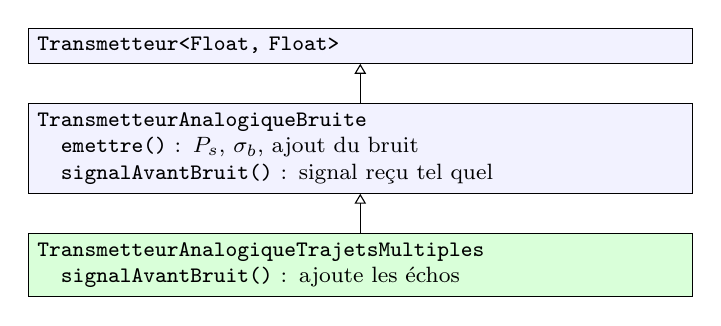
\begin{tikzpicture}[b/.style={draw,align=left,font=\footnotesize,fill=blue!5,text width=8.2cm},>=Stealth]
\node[b] (t) {\texttt{Transmetteur<Float, Float>}};
\node[b,below=0.5cm of t] (b) {\texttt{TransmetteurAnalogiqueBruite}\\\quad\texttt{emettre()} : $P_s$, $\sigma_b$, ajout du bruit\\\quad\texttt{signalAvantBruit()} : signal reçu tel quel};
\node[b,below=0.5cm of b,fill=green!15] (m) {\texttt{TransmetteurAnalogiqueTrajetsMultiples}\\\quad\texttt{signalAvantBruit()} : ajoute les échos};
\draw[-{Triangle[open]}] (b)--(t); \draw[-{Triangle[open]}] (m)--(b);
\end{tikzpicture}\end{center}
\begin{lstlisting}
// TransmetteurAnalogiqueBruite.emettre() (extrait simplifié)
float[] signal = signalAvantBruit();            // point d'extension
double ps = sommeCarres(signal) / n;            // puissance mesurée après les échos
double sigmaB2 = (ps * nbEch) / (2.0 * ebN0Lineaire);
for (int i = 0; i < n; i++)
    informationEmise.add((float) (signal[i] + genererBruitGaussien(sigmaB)));

// TransmetteurAnalogiqueTrajetsMultiples
@Override
protected float[] signalAvantBruit() {
    for (int i = 0; i < n; i++) {
        float valeur = informationRecue.iemeElement(i);
        for (int k = 0; k < retards.length; k++)
            if (i - retards[k] >= 0)
                valeur += amplitudes[k] * informationRecue.iemeElement(i - retards[k]);
        avecTrajets[i] = valeur;
    }
    return avecTrajets;
}
\end{lstlisting}
Conséquences :
\begin{itemize}
  \item la formule du bruit n'existe qu'à un seul endroit, ce qui garantit qu'un même \texttt{-snrpb} donne le même bruit dans les deux canaux ;
  \item conformément à la fiche de la séance 4, $P_s = \frac1N\sum s_{tj}^2$ est mesurée sur le signal \emph{avec échos} ;
  \item sans \texttt{-snrpb}, le simulateur transmet $\EbNo = +\infty$ : on obtient alors $\sigma_b = 0$ et aucun bruit n'est ajouté (étape 4a), sans aucun cas particulier dans le code.
\end{itemize}

\subsection{Défauts corrigés dans la première version}
La première version du canal (commit « Ajout du signal bruité ») a été relue et confrontée à la commande unique. Cinq défauts ont été corrigés :
\begin{center}\small\begin{tabularx}{\linewidth}{>{\raggedright\arraybackslash}p{4.3cm}Xl}\toprule
Défaut & Effet mesuré & Correction\\\midrule
Option \texttt{-trajets n ar dt ...} & refus des commandes de l'enseignant (\texttt{-ti}) & syntaxe \texttt{-ti dt ar}\\
Condition \texttt{canalBruite} testée deux fois & \texttt{-trajets} sans effet & branchement corrigé\\
$\EbNo$ par défaut à 0~dB & écho $dt = N$, $ar = 0{,}5$, sans \texttt{-snrpb} (NRZ $\pm1$, $N = 10$) : TEB $0{,}150$ au lieu de 0 & $\EbNo = +\infty$\\
Facteur $N$ oublié dans $\sigma_b^2$ (copie de la formule) & bruit 30 fois trop faible : écho nul, 0~dB (NRZ $0/1$), TEB $0{,}158$ au lieu de $0{,}428$ & héritage\\
Retard négatif accepté & accès hors du tableau & refusé\\\bottomrule
\end{tabularx}\end{center}
Le troisième défaut rendait un test JUnit trompeur : « TEB non nul avec \texttt{-trajets} sans \texttt{-snrpb} » ne réussissait que grâce au bruit caché. Il a été remplacé par deux tests, l'un avec des échos réellement destructeurs, l'autre vérifiant qu'un écho faible sans bruit donne un TEB nul.

%======================================================================
\section{Récepteur à filtre adapté}\label{sec:filtre}
\subsection{Principe}
Pour une impulsion $p(t)$ de durée $T$ reçue dans un bruit blanc gaussien, le filtre linéaire qui maximise le rapport signal à bruit à l'instant de décision est le \textbf{filtre adapté}, de réponse impulsionnelle $h(t) = p(T-t)$ : l'impulsion retournée dans le temps et décalée pour être causale~[1]. Échantillonnée en $t = T$, sa sortie est une \textbf{corrélation} :
\[ y(T) = \int r(\tau)\,h(T-\tau)\,d\tau = \int_0^T r(\tau)\,p(\tau)\,d\tau . \]
Le signal utile s'additionne de façon cohérente sur tout le bit, alors que le bruit, indépendant d'un échantillon à l'autre, se moyenne. C'est précisément ce que ne faisait pas le récepteur de l'étape 3, qui n'utilisait qu'un échantillon sur $N$.

\subsection{Une règle de décision unique pour les trois formes d'onde}
Notons $s_1$ et $s_0$ les $N$ échantillons d'un bit 1 et d'un bit 0, et $r$ les échantillons reçus pendant un bit. Avec un bruit gaussien, la décision optimale choisit le symbole le plus proche :
\[ \|r - s_1\|^2 < \|r - s_0\|^2 \iff \underbrace{\sum_{k=0}^{N-1} r[k]\, g[k]}_{y} > \underbrace{\frac{\|s_1\|^2 - \|s_0\|^2}{2}}_{\text{seuil}}, \qquad g = s_1 - s_0 . \]
C'est un filtre adapté à la \emph{différence} $g$ des deux symboles. La forme d'onde n'apparaît que dans $g$ : la même formule convient à NRZ, NRZT et RZ, et le seuil s'en déduit automatiquement (figure~\ref{fig:filtres}) :
\begin{itemize}
  \item \textbf{NRZ} : $g$ est constant, $y$ est la somme des échantillons du bit ; ramené à une moyenne, le seuil vaut $(A_{\min}+A_{\max})/2$ comme à l'étape 3 ;
  \item \textbf{RZ} : $g$ est nul hors du tiers central, qui ne contient que du bruit ; le filtre l'ignore ;
  \item \textbf{NRZT} : les échantillons des rampes, moins fiables, reçoivent un poids plus faible.
\end{itemize}
\begin{figure}[htbp]\centering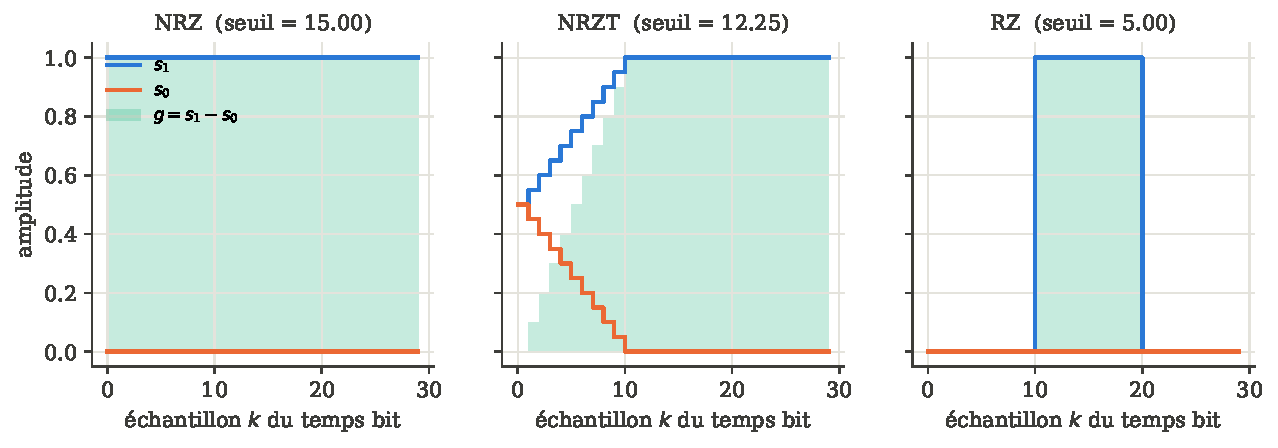
\includegraphics[width=\linewidth]{figures/fig_filtres.pdf}
\caption{Formes de référence $s_1$, $s_0$ et filtre $g = s_1 - s_0$ pour $N = 30$ et les amplitudes $(0, 1)$. Le seuil est exprimé en unités de la somme $y$.}\label{fig:filtres}\end{figure}

\subsection{Cas du NRZT}
Dans notre émetteur, la rampe d'un bit part du niveau du bit précédent : un bit 1 précédé d'un 1 est plat, précédé d'un 0 il commence par une rampe montante. Le symbole n'est donc pas unique. Nous prenons pour $s_1$ et $s_0$ la \textbf{moyenne sur les deux valeurs possibles du bit précédent}. La partie qui dépend du bit précédent s'annule alors dans $g$ : sur la rampe, $g[k] = (A_{\max} - A_{\min})\,k/t_1$, qui ne dépend que du bit courant. Le filtre n'est plus strictement optimal (le bit précédent crée une petite IES), mais la marge reste largement positive : sans bruit, toute séquence est décodée sans erreur.

\subsection{Implémentation}
Pour ne pas coder deux fois les formes d'onde, le récepteur demande $s_1$ et $s_0$ à l'émetteur, via la méthode \texttt{formeBit} extraite de \cls{TransmetteurLogiqueAnalogique}. Le filtre et le seuil sont calculés une fois, à la construction :
\begin{lstlisting}
public TransmetteurAnalogiqueLogique(String forme, int nbEch, float aMin, float aMax) {
    for (boolean bitPrecedent : new boolean[] {false, true}) {   // moyenne (NRZT)
        float[] un   = TransmetteurLogiqueAnalogique.formeBit(forme, nbEch, aMin, aMax, true,  bitPrecedent);
        float[] zero = TransmetteurLogiqueAnalogique.formeBit(forme, nbEch, aMin, aMax, false, bitPrecedent);
        for (int k = 0; k < nbEch; k++) { s1[k] += un[k] / 2f;  s0[k] += zero[k] / 2f; }
    }
    for (int k = 0; k < nbEch; k++) {
        filtre[k] = s1[k] - s0[k];
        seuil += filtre[k] * (s1[k] + s0[k]) / 2.0;   // = (||s1||^2 - ||s0||^2) / 2
    }
}

public void emettre() {
    for (int i = 0; i < nbBits; i++) {
        double y = 0.0;
        for (int k = 0; k < nbEch; k++)
            y += informationRecue.iemeElement(i * nbEch + k) * filtre[k];
        informationEmise.add(y > seuil);
    }
}
\end{lstlisting}
Une nouvelle forme d'onde ajoutée à l'émetteur serait donc prise en charge par le récepteur sans modification. La commande unique ne change pas : le récepteur est choisi à partir de \texttt{-form}, \texttt{-nbEch} et \texttt{-ampl}, déjà connus du simulateur.

\subsection{TEB théorique}\label{sec:theorie}
En sortie du filtre, le bruit est gaussien d'écart-type $\sigma_b\|g\|$, avec $\sigma_b^2 = P_s N / (2\,\EbNo)$ (étape 3). En l'absence d'IES :
\[ \text{TEB} = Q\!\left(\frac{\|s_1 - s_0\|}{2\sigma_b}\right). \]
\begin{center}\begin{tabular}{lccc}\toprule
Forme & $P_s$ & $\|s_1 - s_0\|^2$ & TEB (filtre adapté)\\\midrule
NRZ antipodal $(-A, A)$ & $A^2$ & $4A^2N$ & $Q\big(\sqrt{2\EbNo}\big)$\\
NRZ unipolaire $(0, A)$ & $A^2/2$ & $A^2N$ & $Q\big(\sqrt{\EbNo}\big)$\\
RZ unipolaire $(0, A)$ & $A^2/6$ & $A^2N/3$ & $Q\big(\sqrt{\EbNo}\big)$\\
RZ antipodal $(-A, A)$ & $A^2$ & $4A^2N/3$ & $Q\big(\sqrt{2\EbNo/3}\big)$\\\bottomrule
\end{tabular}\end{center}
Pour le NRZT, et pour tous les cas avec échos, l'IES rend le TEB dépendant des bits voisins. Le script \texttt{courbesTEB.py} calcule alors une \textbf{théorie exacte} : il énumère toutes les suites possibles des bits voisins (le précédent pour la rampe, ceux qu'atteignent les échos), reconstruit la fenêtre reçue sans bruit avec les mêmes formes que l'émetteur, calcule $P_s$ sur ce signal avec échos, puis moyenne $Q(\text{marge}/\sigma_y)$ sur toutes les suites. Le même calcul, avec $y = r[N/2]$ et $\sigma_y = \sigma_b$, donne la théorie du récepteur de l'étape 3.

%======================================================================
\section{Résultats}
Toutes les courbes sont produites par \texttt{rapport/etape4/courbesTEB.py}, avec $N = 30$. Les points sont simulés par notre simulateur (jusqu'à $10^6$ bits par point, en tranches de 200\,000 bits avec des semences différentes) ; les traits sont la théorie exacte de la section~\ref{sec:theorie}. Les points à TEB nul ne sont pas représentés.

\subsection{Filtre adapté : conformité à la théorie}
\begin{figure}[htbp]\centering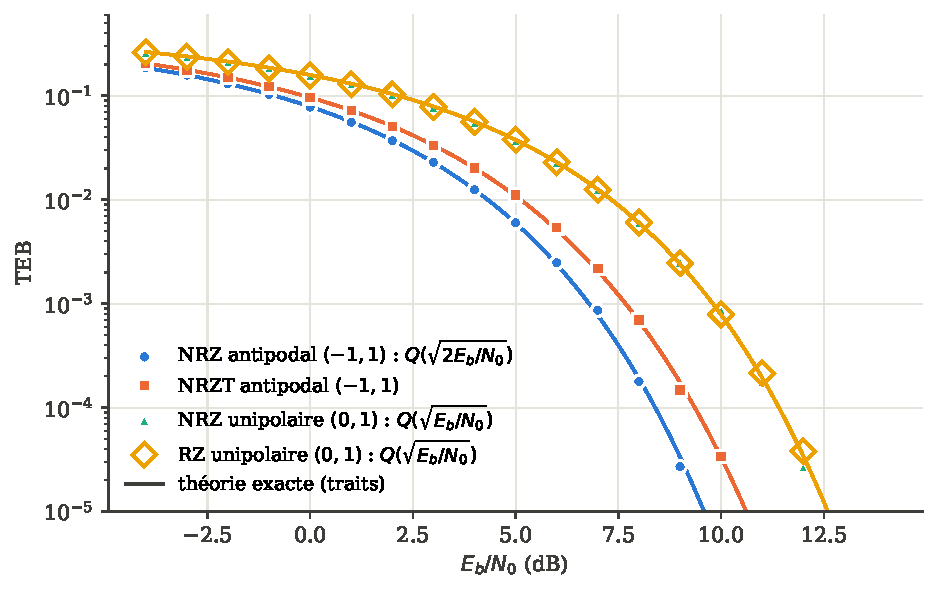
\includegraphics[width=0.85\linewidth]{figures/fig_teb_filtre.pdf}
\caption{TEB du récepteur à filtre adapté (points) et théorie exacte (traits), canal gaussien sans écho.}\label{fig:tebfiltre}\end{figure}
Les points simulés se superposent à la théorie sur plus de quatre décades, jusqu'à $3\cdot10^{-5}$. L'écart médian entre simulation et théorie est de 0,8\,\%. L'écart relatif maximal (12\,\%) concerne des points à environ 170 erreurs, dont l'incertitude statistique relative est de l'ordre de $1/\sqrt{170} \approx 8\,\%$ : il représente 1,5 écart-type. Sur les 313 points simulés pour ce rapport, aucun ne s'écarte de la théorie de plus de 2,5 écarts-types (loi binomiale), ce qui est conforme à des fluctuations purement statistiques.
\begin{center}\begin{tabular}{lcccc}\toprule
& \multicolumn{2}{c}{4 dB} & \multicolumn{2}{c}{8 dB}\\
Configuration & simulé & théorie & simulé & théorie\\\midrule
NRZ antipodal $(-1,1)$ & $1{,}25\cdot10^{-2}$ & $1{,}25\cdot10^{-2}$ & $1{,}78\cdot10^{-4}$ & $1{,}91\cdot10^{-4}$\\
NRZT antipodal $(-1,1)$ & $2{,}01\cdot10^{-2}$ & $2{,}01\cdot10^{-2}$ & $7{,}0\cdot10^{-4}$ & $6{,}8\cdot10^{-4}$\\
NRZ unipolaire $(0,1)$ & $5{,}60\cdot10^{-2}$ & $5{,}65\cdot10^{-2}$ & $6{,}09\cdot10^{-3}$ & $6{,}00\cdot10^{-3}$\\
RZ unipolaire $(0,1)$ & $5{,}63\cdot10^{-2}$ & $5{,}65\cdot10^{-2}$ & $6{,}03\cdot10^{-3}$ & $6{,}00\cdot10^{-3}$\\\bottomrule
\end{tabular}\end{center}
Le NRZ unipolaire et le RZ unipolaire ont exactement la même courbe : avec le filtre adapté, seule compte l'énergie de la différence $s_1 - s_0$ rapportée à $E_b$, identique dans les deux cas (tableau de la section~\ref{sec:theorie}). Le NRZT perd environ 0,9~dB sur le NRZ : les rampes réduisent l'énergie utile de $g$ et le bit précédent crée une légère IES.

\subsection{Gain par rapport à l'étape 3}
\begin{figure}[htbp]\centering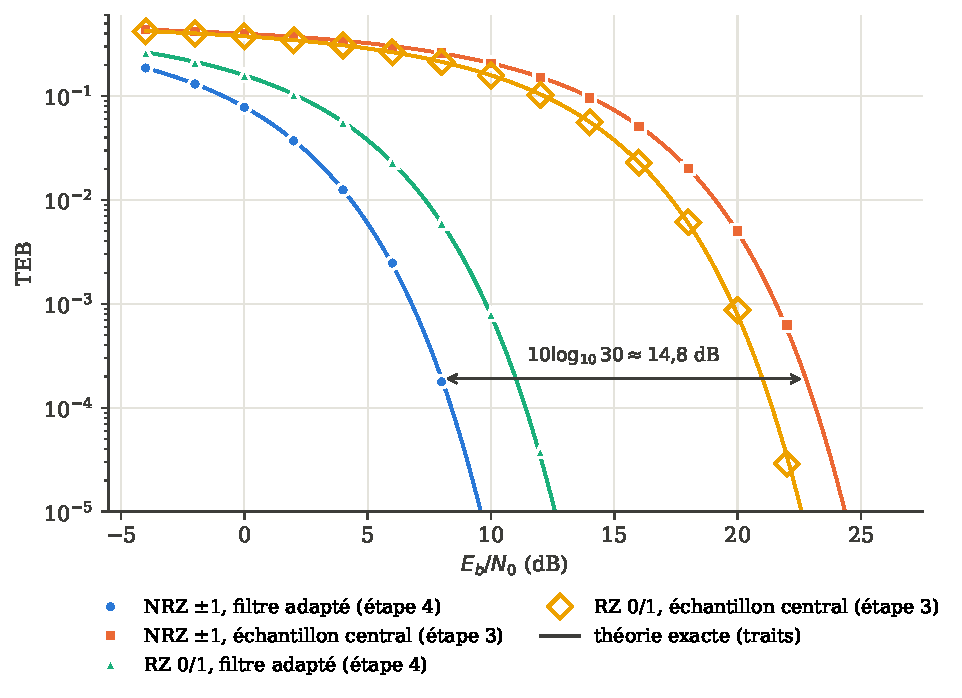
\includegraphics[width=0.85\linewidth]{figures/fig_avant_apres.pdf}
\caption{Récepteur de l'étape 3 (échantillon central, recompilé depuis le commit \texttt{82e4660}) et récepteur à filtre adapté.}\label{fig:avantapres}\end{figure}
Le récepteur de l'étape 3 a été recompilé à partir du commit qui le contient encore et soumis aux mêmes balayages. Ses mesures suivent la théorie de la décision sur un échantillon ($0{,}258$ mesuré et théorique à 8~dB en NRZ). Le tableau donne le $\EbNo$ nécessaire pour atteindre un TEB de $10^{-3}$ (théorie exacte, confirmée par les points simulés) :
\begin{center}\begin{tabular}{lccc}\toprule
Forme & Étape 3 (échantillon central) & Étape 4 (filtre adapté) & Gain\\\midrule
NRZ antipodal $(-1,1)$ & 21,6 dB & 6,8 dB & \textbf{14,8 dB}\\
NRZT antipodal $(-1,1)$ & 21,1 dB & 7,7 dB & \textbf{13,4 dB}\\
RZ unipolaire $(0,1)$ & 19,8 dB & 9,8 dB & \textbf{10,0 dB}\\\bottomrule
\end{tabular}\end{center}
Le gain vaut $10\log_{10}M$, où $M$ est le nombre d'échantillons qui portent l'information : $M = N = 30$ en NRZ (14,8~dB), mais seulement $M = N/3 = 10$ en RZ (10~dB), dont seul le tiers central distingue un 1 d'un 0. En NRZT, les rampes rendent une partie des échantillons moins utiles, d'où un gain intermédiaire. Le RZ, qui paraissait meilleur que le NRZ à l'étape 3 (artefact de la décision ponctuelle, déjà expliqué dans le rapport précédent), retrouve sa place théorique : 3~dB derrière le NRZ antipodal.

\subsection{Trajets multiples sans bruit (étape 4a)}
\begin{figure}[htbp]\centering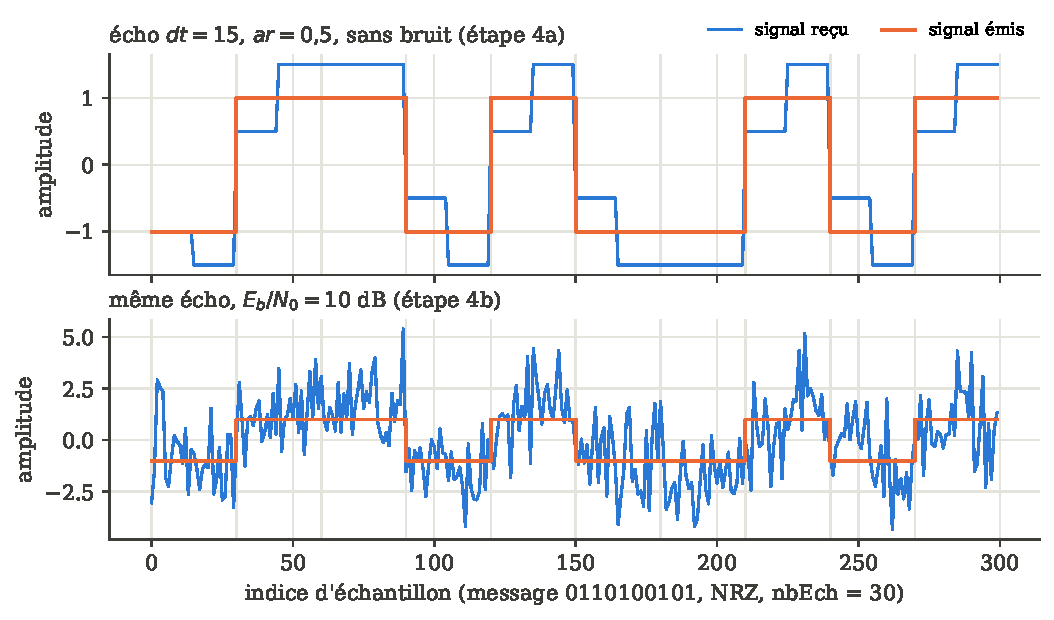
\includegraphics[width=0.9\linewidth]{figures/fig_signal_echo.pdf}
\caption{Signal NRZ $(-1, 1)$ émis et reçu avec un écho $dt = 15$, $ar = 0{,}5$ (sortie des classes du simulateur via \texttt{ExportSignal}).}\label{fig:signal}\end{figure}
La figure~\ref{fig:signal} montre l'effet d'un écho retardé d'un demi-bit : la première moitié de chaque bit reçoit l'écho du bit précédent, la seconde celui du bit courant. Quand deux bits consécutifs sont égaux, l'écho renforce le signal ($1{,}5$) ; quand ils diffèrent, il l'atténue ($0{,}5$) sur la première moitié du bit.
\begin{figure}[htbp]\centering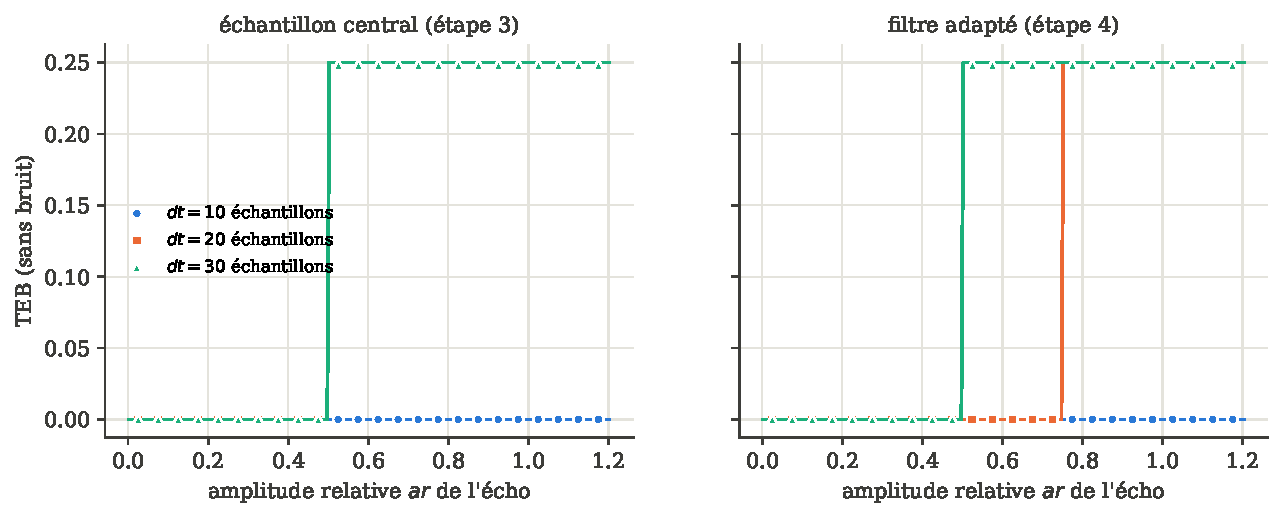
\includegraphics[width=\linewidth]{figures/fig_trajets_alpha.pdf}
\caption{TEB sans bruit en fonction de l'amplitude de l'écho, NRZ unipolaire $(0,1)$ (amplitudes par défaut), un seul trajet indirect, 20\,000 bits par point. Pour $dt = 20$, la courbe de l'étape 3 est confondue avec celle de $dt = 30$.}\label{fig:alpha}\end{figure}
Sans bruit, le TEB est soit nul, soit égal à $1/4$ : toutes les erreurs viennent d'une même configuration, un bit 0 précédé d'un bit 1, dont l'écho fait franchir le seuil. Pour le NRZ unipolaire avec un écho $dt \le N$, la sortie du filtre adapté (ici $g = 1$, seuil $N/2$) se calcule directement. Les $dt$ premiers échantillons du bit courant $b$ reçoivent l'écho du bit précédent $p$, les autres celui du bit courant :
\[ y = \sum_{k<dt}(b + ar\,p) + \sum_{k\ge dt}(b + ar\,b) = N b + ar\,\big(dt\, p + (N - dt)\,b\big). \]
Pour $b = 0$ et $p = 1$, $y = ar\,dt$ dépasse le seuil $N/2$ dès que $ar > N/(2\,dt)$. Cette configuration a une probabilité $1/4$ :
\begin{center}\small\begin{tabularx}{\linewidth}{c>{\centering\arraybackslash}X>{\centering\arraybackslash}X>{\centering\arraybackslash}X}\toprule
$dt$ & seuil d'erreur, filtre adapté & mesuré (filtre adapté) & seuil d'erreur, étape 3\\\midrule
10 & $ar > 1{,}5$ & aucune erreur jusqu'à 1,175 (fin du balayage) & jamais (l'échantillon central voit l'écho du bit courant)\\
20 & $ar > 0{,}75$ & premières erreurs à 0,775 & $ar > 0{,}5$\\
30 & $ar > 0{,}5$ & premières erreurs à 0,525 & $ar > 0{,}5$\\\bottomrule
\end{tabularx}\end{center}
Le filtre adapté résiste mieux à un écho qui ne recouvre qu'une partie du bit ($dt = 20$) : il moyenne l'écho du bit précédent avec la partie saine du bit, alors que l'échantillon central tombe en plein dans l'écho. Pour un écho d'un bit entier ($dt = N$), les deux récepteurs sont équivalents. En NRZ antipodal $(-1, 1)$, le seuil est à 0 et, pour tout retard, $y \cdot \text{signe}(b) \ge N(1 - ar)$ : il faut $ar > 1$ pour une erreur, ce qui est physiquement exclu pour un trajet indirect ($ar < 1$) : c'est pourquoi le test JUnit des échos destructeurs utilise deux échos de $0{,}9$ qui s'additionnent.

\subsection{Trajets multiples et bruit (étape 4b)}
\begin{figure}[htbp]\centering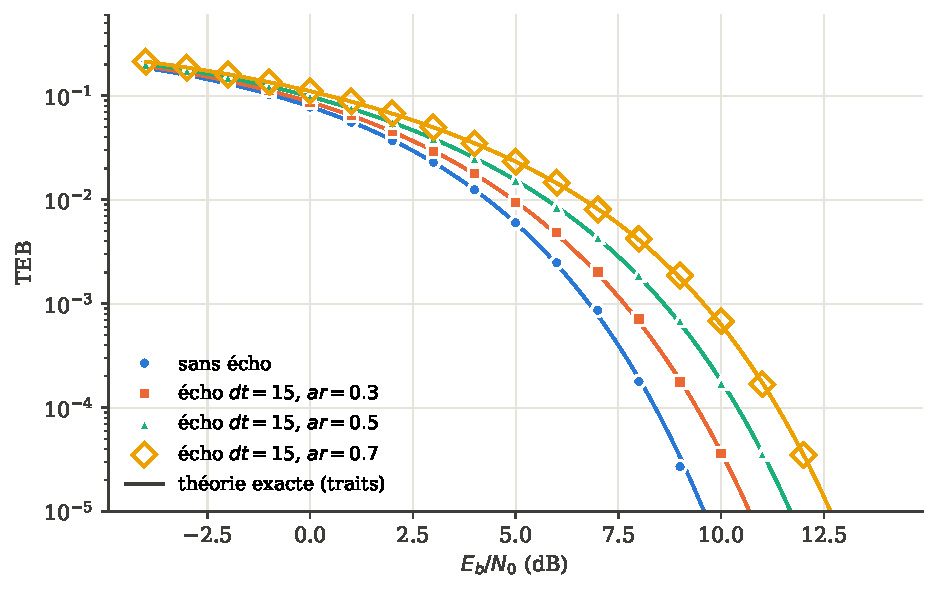
\includegraphics[width=0.85\linewidth]{figures/fig_trajets_ebn0.pdf}
\caption{TEB en présence d'un écho $dt = 15$ (un demi-bit) et de bruit, NRZ antipodal $(-1, 1)$, filtre adapté.}\label{fig:ebn0}\end{figure}
Pour un écho d'un demi-bit en NRZ antipodal, le calcul de la section précédente donne deux cas équiprobables :
\begin{itemize}
  \item bits précédent et courant égaux : l'écho renforce tout le bit, la marge est multipliée par $(1 + ar)$ ;
  \item bits différents : l'écho du bit précédent et celui du bit courant se compensent exactement, la marge est celle d'un canal sans écho.
\end{itemize}
Mais la puissance reçue augmente, $P_s = \frac34(1 + ar)^2 + \frac14(1 - ar)^2$, et le bruit, réglé sur $E_b = P_s T$ mesuré après les échos (fiche de la séance 4), augmente dans la même proportion :
\[ \text{TEB} = \tfrac12\,Q\Big(\sqrt{2\EbNo / P_s}\Big) + \tfrac12\,Q\Big((1 + ar)\sqrt{2\EbNo / P_s}\Big). \]
\begin{center}\begin{tabular}{ccccc}\toprule
$ar$ & TEB à 8 dB (simulé) & TEB à 8 dB (théorie) & $\EbNo$ pour $10^{-3}$ & pénalité\\\midrule
0 & $1{,}78\cdot10^{-4}$ & $1{,}91\cdot10^{-4}$ & 6,8 dB & --\\
0,3 & $7{,}2\cdot10^{-4}$ & $6{,}7\cdot10^{-4}$ & 7,6 dB & 0,9 dB\\
0,5 & $1{,}88\cdot10^{-3}$ & $1{,}83\cdot10^{-3}$ & 8,6 dB & 1,8 dB\\
0,7 & $4{,}2\cdot10^{-3}$ & $4{,}1\cdot10^{-3}$ & 9,6 dB & 2,8 dB\\\bottomrule
\end{tabular}\end{center}
La pénalité reste inférieure à l'augmentation de puissance $10\log_{10}P_s$ (1,4 ; 2,4 ; 3,4~dB) : la moitié du temps, l'écho renforce la décision, ce qui compense en partie.

%======================================================================
\section{Confrontation aux prévisions}
\subsection{Ce qui est conforme}
\begin{itemize}
  \item \textbf{Filtre adapté} : le TEB rejoint la borne optimale ($1{,}25\cdot10^{-2}$ à 4~dB en NRZ antipodal, simulé et théorique) et le gain prévu de 14,8~dB est mesuré. Les 3~dB entre antipodal et unipolaire sont retrouvés.
  \item \textbf{Trajets multiples sans bruit} : le TEB est nul tant que l'écho ne fait pas franchir le seuil, puis vaut exactement la probabilité des suites défavorables ($1/4$). Les seuils d'apparition des erreurs mesurés correspondent au calcul ($ar > N/(2\,dt)$).
  \item \textbf{Trajets multiples et bruit} : le TEB augmente avec $ar$ à $\EbNo$ fixé, et la théorie exacte prédit chaque point.
\end{itemize}
\subsection{Ce qui diffère de l'intuition}
\begin{itemize}
  \item L'écho d'un bit entier est bien le plus gênant, mais seulement pour les amplitudes unipolaires, dont le seuil est à mi-hauteur : il provoque des erreurs dès $ar > 0{,}5$. En NRZ antipodal, un écho \emph{unique} d'amplitude $ar < 1$ ne crée jamais d'erreur sans bruit, quel que soit son retard ; il faut plusieurs échos qui s'additionnent.
  \item En 4b, une partie de la dégradation vient de la définition de $\EbNo$ : l'énergie de l'écho est comptée dans $E_b$ alors qu'elle n'est utile que la moitié du temps.
  \item Le RZ est robuste aux échos courts : son impulsion est concentrée dans le tiers central, et l'écho de l'impulsion précédente n'atteint le tiers central du bit courant que si $dt > 2N/3$. Vérifié par simulation (RZ $0/1$, 20\,000 bits, sans bruit) : aucune erreur pour $dt \in \{10, 15, 20\}$ jusqu'à $ar = 1{,}1$, alors qu'à $dt = 30$ le TEB vaut $0{,}25$ dès $ar = 0{,}7$.
\end{itemize}

%======================================================================
\section{Tests}
\subsection{Tests automatiques (\texttt{runTests})}
Le script couvre maintenant les étapes 1 à 4 dans des sections séparées ; chaque commentaire \texttt{\# Test n} correspond au numéro affiché. Six tests concernent l'étape 4 :
\begin{lstlisting}[language={}]
Test 15 : Trajets indirects (1 trajet, sans bruit) ... OK
Test 16 : Trajets indirects (1 trajet, bruité) ... OK
Test 17 : Trajets indirects (3 trajets, bruité) ... OK
Test 26 : Erreur (ti sans couple) ... OK
Test 27 : Erreur (ti sans valeur ar) ... OK
Test 28 : Erreur (ti plus de 5 couples) ... OK
------------------------------------------
  RÉSULTAT : 28/28 OK
\end{lstlisting}

\subsection{Tests unitaires JUnit}
La suite passe de 75 à \textbf{96 tests} (22 ajoutés, 1 supprimé), tous réussis. Tests ajoutés :
\begin{itemize}
  \item \textbf{canal à trajets multiples} (\cls{TransmetteurTest}, préfixe TATM) : écho appliqué seulement après son retard ; bruit reproductible avec une semence ; signal vide ; \emph{bruit identique à celui du canal gaussien sans trajet indirect} (vérifie le partage de la formule) ; rejet de tableaux incohérents, de plus de 5 trajets et d'un retard négatif ;
  \item \textbf{filtre adapté} (préfixe TAL) : en RZ, une forte perturbation hors du tiers central ne change pas la décision ; un échantillon central très faussé ne suffit plus à provoquer une erreur ; une séquence NRZT avec toutes les combinaisons de rampes est décodée sans erreur ;
  \item \textbf{simulateur} : \texttt{-ti} avec des échos destructeurs donne un TEB non nul ; \texttt{-ti} sans \texttt{-snrpb} n'ajoute pas de bruit ; un écho d'amplitude nulle donne exactement le même TEB que \texttt{-snrpb} seul ; \texttt{-ti} suivi d'autres options ; rejets des valeurs invalides ; \emph{TEB conforme à la théorie} : NRZ antipodal à 4~dB, $1{,}25\cdot10^{-2}$ à $\pm 12\,\%$ sur $10^5$ bits ;
  \item compléments de couverture ajoutés par L.~Nanda sur l'émetteur (rampes NRZT, forme inconnue, signal vide) et le canal gaussien.
\end{itemize}
Le dernier test simulateur répond à la limite relevée à l'étape 3 : les tests vérifiaient que le simulateur affichait un TEB, pas sa valeur.

\subsection{Limites identifiées}
\begin{itemize}
  \item \textbf{Semences liées.} Avec \texttt{-seed}, la source et le canal utilisent toujours la même semence, donc des suites pseudo-aléatoires liées. Utiliser \texttt{seed} et \texttt{seed + 1} garantirait leur indépendance. Les courbes restent conformes à la théorie, ce qui indique que l'effet est négligeable ici.
  \item \textbf{Mémoire.} \cls{Information} stocke des \texttt{Float} (objets) : une simulation de 200\,000 bits à 30 échantillons occupe environ 400~Mo. Les balayages sont donc découpés en tranches ; un stockage en \texttt{float[]} réduirait fortement l'empreinte.
  \item \textbf{Pas de compensation des échos.} Le filtre adapté est optimal contre le bruit, pas contre l'IES. Un égaliseur est nécessaire pour annuler les trajets multiples.
  \item Le rapport de l'étape 3 prévoyait une option pour conserver la décision sur l'échantillon central. La commande unique n'en prévoyant pas, la comparaison est faite en recompilant la version de l'étape 3 depuis git (script de courbes).
\end{itemize}

%======================================================================
\section{Conclusion}
Le canal à trajets multiples est intégré au simulateur avec l'option \texttt{-ti} de la commande unique, avec ou sans bruit. L'héritage de \cls{TransmetteurAnalogiqueBruite} garantit que le bruit est calculé de la même façon dans les deux canaux, ce qui a supprimé une erreur de facteur $N$ présente dans la première version.

Le récepteur à filtre adapté, annoncé comme prioritaire à la fin de l'étape 3, est en place. Une seule règle, la corrélation avec $g = s_1 - s_0$, sert aux trois formes d'onde. Le TEB mesuré atteint désormais la borne théorique, soit un gain de 14,8~dB en NRZ et 10~dB en RZ par rapport à l'étape 3. Toutes les mesures, avec ou sans échos, sont prédites par une théorie exacte de la chaîne, avec un écart médian inférieur à 1\,\%.

Le filtre adapté ne compense pas les échos : en présence de trajets multiples, le TEB reste dégradé (1,8~dB de pénalité pour un écho de 0,5 à un demi-bit) et, sans bruit, un écho fort impose un TEB de $1/4$ en unipolaire. Deux pistes pour la suite : un égaliseur, qui estime et soustrait l'écho des bits déjà décidés, et le codage de canal de l'étape 5, qui pourra maintenant être évalué sur un récepteur optimal.

\section*{Annexe -- Reproduire les figures}
\begin{lstlisting}[language={}]
./compile
python3 rapport/etape4/courbesTEB.py               # réutilise les données de rapport/etape4/donnees/
python3 rapport/etape4/courbesTEB.py --recalculer  # relance les simulations (quelques minutes)
\end{lstlisting}
Les valeurs de chaque point (commande, nombre de bits, TEB simulé et théorique) sont enregistrées au format CSV dans \texttt{rapport/etape4/donnees/}.

\section*{Références}
\begin{enumerate}\small
\item[{[1]}] J. G. Proakis, M. Salehi, \emph{Digital Communications}, 5e éd., McGraw-Hill, 2008 -- chap. 4 (détection optimale, filtre adapté) et chap. 9 (transmission sur canaux à bande limitée, interférence entre symboles, égalisation).
\item[{[2]}] B. Sklar, \emph{Digital Communications: Fundamentals and Applications}, 2e éd., Prentice Hall, 2001 -- chap. 3 (détection en bande de base, signaux antipodaux et unipolaires).
\item[{[3]}] IMT Atlantique, SIT213 -- fiche de la séance 4 « Canal à trajets multiples et bruité », commande unique du simulateur, énoncé de l'atelier logiciel.
\end{enumerate}
\end{document}
